In order to test the validity of using neural networks sampled
from molecular dynamics trajectories to generate new trajectories
we train neural networks on systems of copper and silicon atoms
using the Effective Medium Theory and Stillinger-Weber potentials
respectively. These potentials have efficient implementations
through ASE and their ASAP interface, which makes
it ideal for our purposes. Additionally these potentials
have an intermediate complexity, with Stillinger-Weber explicitly
including threebody interactions, which makes them ideal
for testing whether the Behler-Parrinello method can replicate this.
At temperatures which are not too large these potentials describe
atoms in a crystalline structure in equilibrium,
and we test whether the neural network can reproduce the correct potential
energy, forces, radial distribution and mean squared displacement.

\begin{table}[h]
\label{tab:hyperparam}
\caption{Hyperparameters used in fitting.}
\begin{center}
\begin{tabular}{|c c|}
\hline
Hyperparameter & Value \\
\hline \hline
Symmetry functions & 16 radial, 24 angular \\
    Hidden layers & $(10, 10)$ \\
Activation & Hyperbolic tangent \\
    Timesteps (fs) & $8 \cdot 10^5$ \\
    Sampling intervall (fs) & 100 \\
Max epochs & 4000 \\
Optimizer & BFGS \\
Energy coefficient & 1.0 \\
Force coefficient & 0.1 \\
\hline
\end{tabular}
\end{center}
\end{table}

\subsection{Effective Medium Theory}
The Effective Medium Theory (EMT) potential gives a good description
of the late transition metals in a Face-Centered Cubic (FCC) crystal
lattice, and has a very efficient implementation in ASE,
which makes it ideal for producing large amounts of data.
We will use a rather small system of $4 \times 2^3 = 32$ atoms
for training, since this means a larger amount of labels available
for atoms when we are only using the potential energy.
We train with only the energy for $8 \cdot 10^5$ steps
with a timestep of $\Delta t = 5.0$ fs
writing to file every 100 steps and then subsequently
train using both energy and forces for $5 \cdot 10^4$ steps
for a total of 500 configurations. We train on both sets of images
for 2000 steps, where the BFGS optimizer has generally converged.
After the calculator is trained we compare the performance
of the neural network with the EMT potential on a system
of 32 atoms with a temperature of 300 Kelvin for 5000 steps.

\begin{figure}[!tbp]
\begin{adjustbox}{max width=1.2\linewidth,center}
\centering
  \begin{subfigure}[b]{0.55\textwidth}
      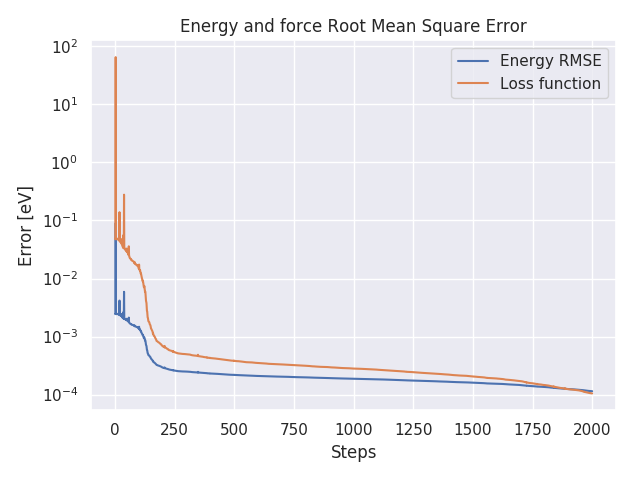
\includegraphics[width=\textwidth]{silicon_energy_log.png}
    \caption{Flower one.}
    \label{fig:f1}
  \end{subfigure}
  \hfill
  \begin{subfigure}[b]{0.55\textwidth}
      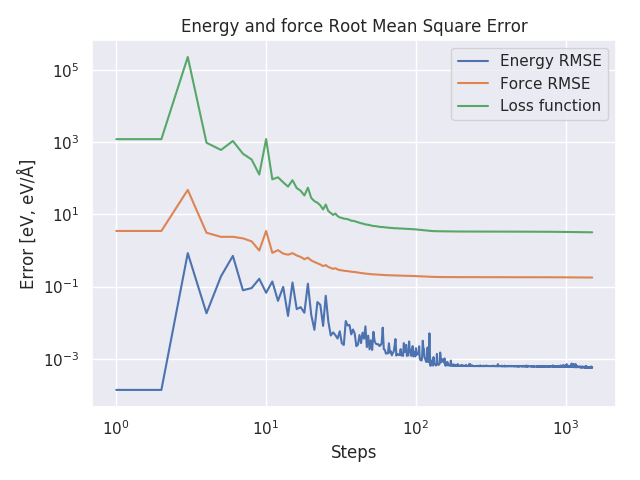
\includegraphics[width=\textwidth]{silicon_force_log.png}
    \caption{Flower two.}
    \label{fig:f2}
  \end{subfigure}
\end{adjustbox}
\caption{My flowers.}
    \label{fig:default}
\end{figure}

\begin{figure}
    \centering
    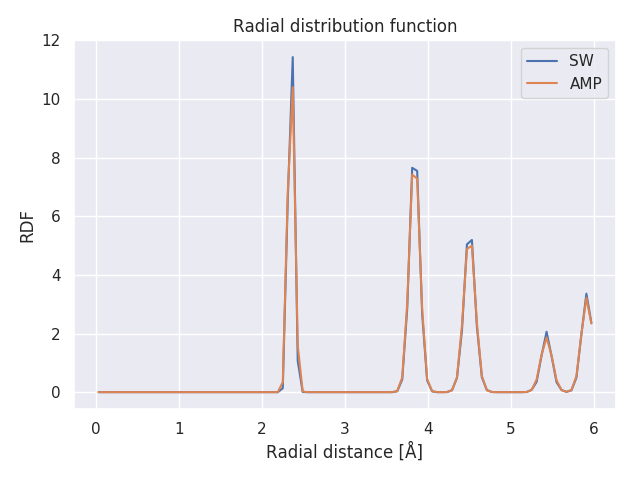
\includegraphics[width=\textwidth]{silicon_rdf.png}
    \caption{Caption}
    \label{fig:silicon-rdf}
\end{figure}

\begin{figure}
    \centering
    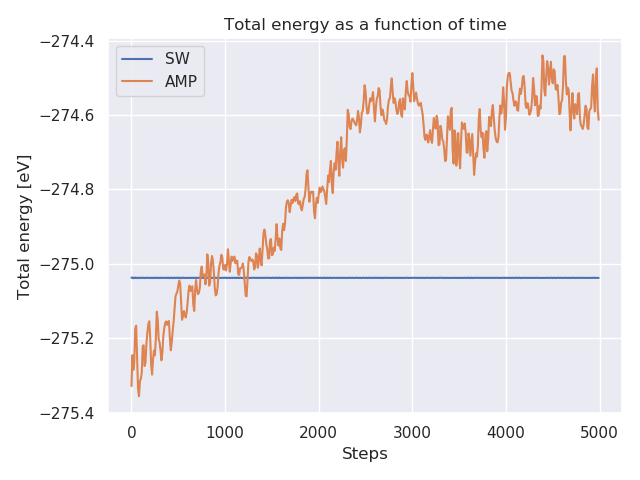
\includegraphics[width=\textwidth]{silicon_energy.png}
    \caption{Caption}
    \label{fig:silicon-energy}
\end{figure}

\begin{figure}
    \centering
    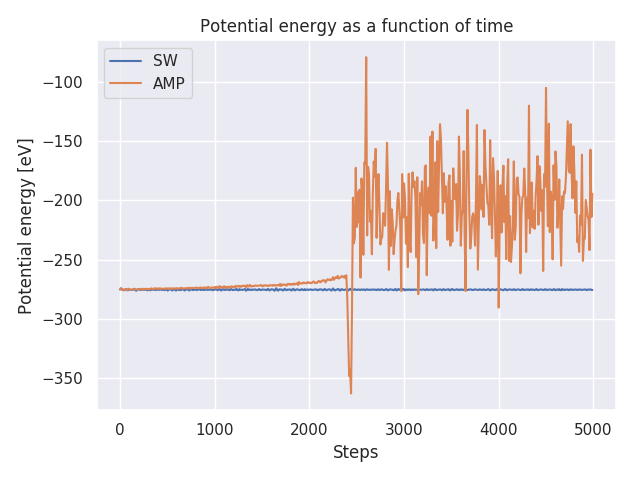
\includegraphics[width=\textwidth]{silicon_pot_energy.png}
    \caption{Caption}
    \label{fig:silicon-energy}
\end{figure}

\begin{figure}
    \centering
    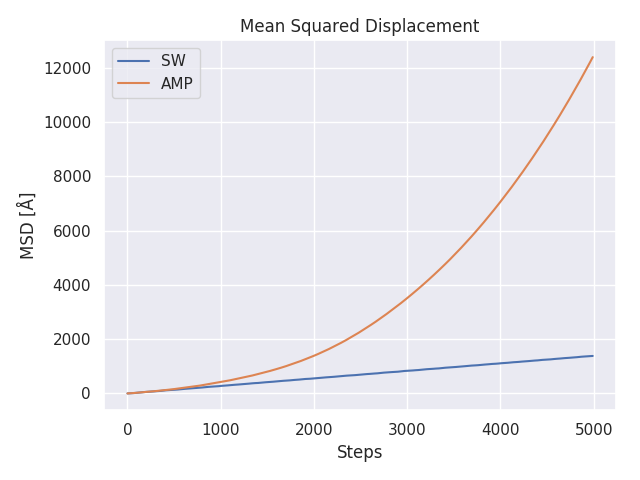
\includegraphics[width=\textwidth]{silicon_msd.png}
    \caption{Caption}
    \label{fig:silicon-energy}
\end{figure}

\subsection{Stillinger-Weber}
The Stillinger-Weber is a potential which describes accurately
Silicon atoms in the diamond lattice structure, and was
one of the first potentials used to describe a realstic atomic-scale
model of Silicon. It is also one of the most common examples
of a potential with a threebody interaction, and its intermediate complexity
makes it ideal for verification with for example quantum calculations
or in our case machine learning methods.
As in the previous section we integrate the system over $8 \cdot 10^5$
steps using a timestep of $\Delta t = 5.0$ fs (suitable for most metals
in a crystalline structure) for a total of 8000 images for energy learning
and 500 images used to train forces. We train for 4000 epochs, since
the loss function is then usually suitably converged.
We generate a test set with identical positions and velocities
using the Stillinger-Weber potential and assess whether the neural network
can accurately reproduce the potential energy, radial distribution function
and more.

\begin{figure}[!tbp]
\begin{adjustbox}{max width=1.2\linewidth,center}
\centering
  \begin{subfigure}[b]{0.55\textwidth}
      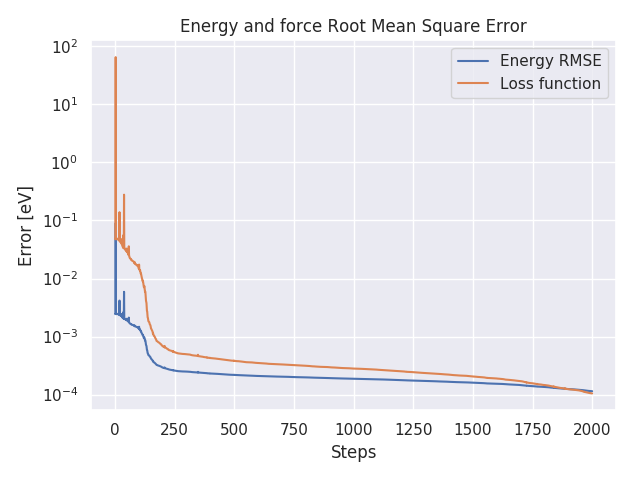
\includegraphics[width=\textwidth]{silicon_energy_log.png}
    \caption{Flower one.}
    \label{fig:f1}
  \end{subfigure}
  \hfill
  \begin{subfigure}[b]{0.55\textwidth}
      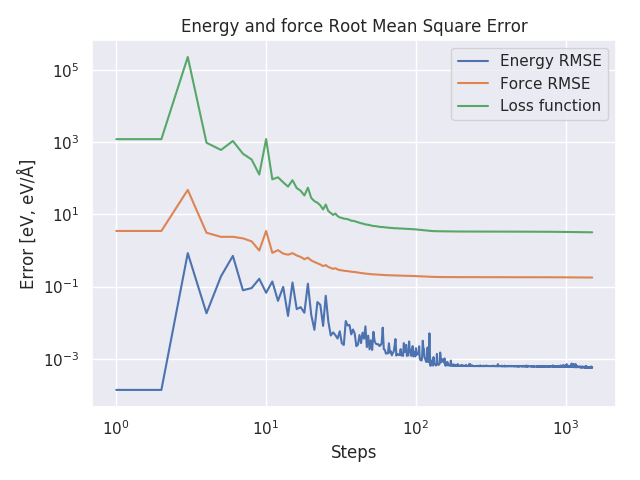
\includegraphics[width=\textwidth]{silicon_force_log.png}
    \caption{Flower two.}
    \label{fig:f2}
  \end{subfigure}
\end{adjustbox}
\caption{My flowers.}
    \label{fig:default}
\end{figure}

\begin{figure}
    \centering
    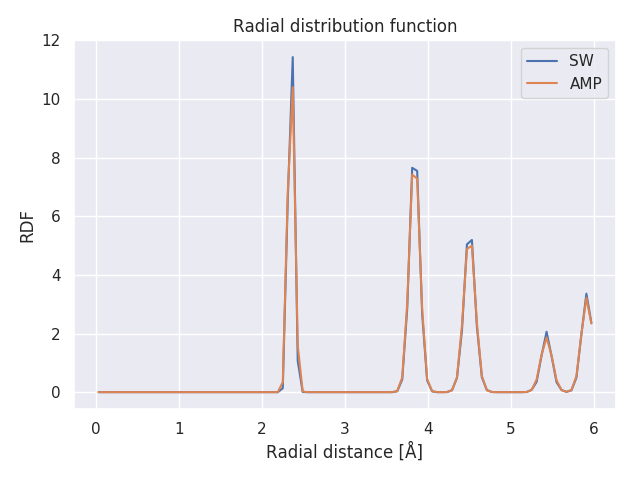
\includegraphics[width=\textwidth]{silicon_rdf.png}
    \caption{Caption}
    \label{fig:silicon-rdf}
\end{figure}

\begin{figure}
    \centering
    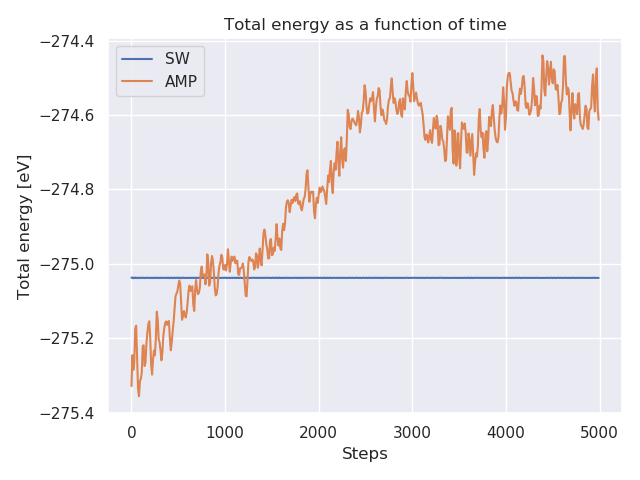
\includegraphics[width=\textwidth]{silicon_energy.png}
    \caption{Caption}
    \label{fig:silicon-energy}
\end{figure}

\begin{figure}
    \centering
    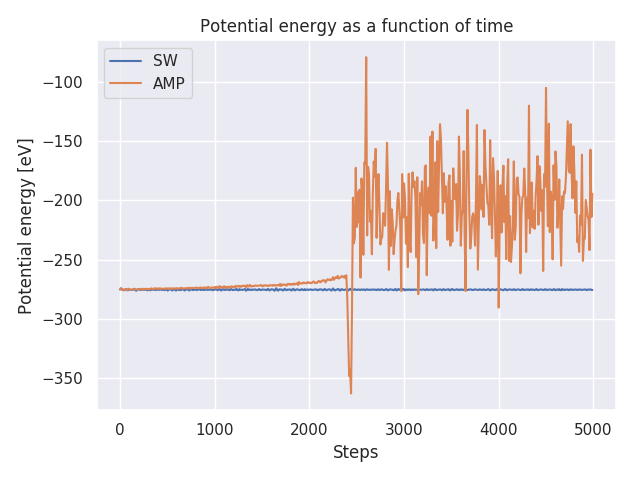
\includegraphics[width=\textwidth]{silicon_pot_energy.png}
    \caption{Caption}
    \label{fig:silicon-energy}
\end{figure}

\begin{figure}
    \centering
    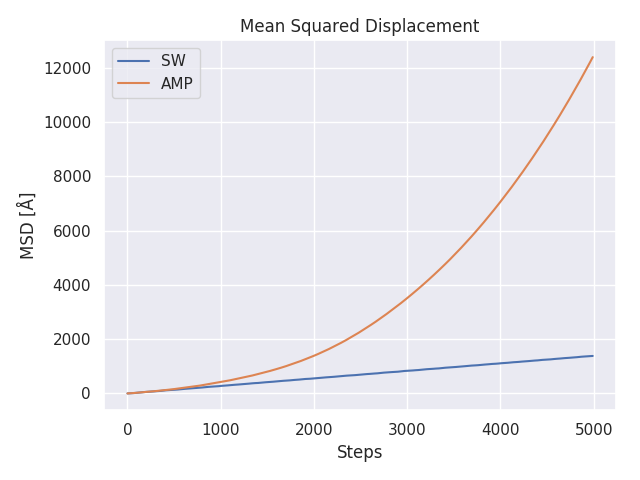
\includegraphics[width=\textwidth]{silicon_msd.png}
    \caption{Caption}
    \label{fig:silicon-energy}
\end{figure}
